% EGL: project presentation (Beamer, 16:9).  Build:  latexmk -pdf egl_slides.tex
% Figures are read from the repository's results/ folder.
\documentclass[aspectratio=169,11pt]{beamer}
\usetheme{default}
\setbeamertemplate{navigation symbols}{}
\setbeamertemplate{footline}{\hfill\scriptsize\color{muted}\insertframenumber\,/\,\inserttotalframenumber\hspace{4mm}\vspace{2.5mm}}
\usepackage{tikz,booktabs,graphicx}
\usetikzlibrary{positioning,arrows.meta,fit,backgrounds,calc}
\graphicspath{{../../results/}{../../results/eval/report/}}

\definecolor{ink}{HTML}{1F2937}
\definecolor{muted}{HTML}{6B7280}
\definecolor{plane}{HTML}{EEF2F7}
\definecolor{ctrl}{HTML}{EAF4EE}
\definecolor{good}{HTML}{1B7F4B}
\definecolor{bad}{HTML}{B42318}
\definecolor{gate}{HTML}{B45309}
\definecolor{blue}{HTML}{1D4ED8}
\setbeamercolor{frametitle}{fg=ink}
\setbeamercolor{normal text}{fg=ink}
\setbeamercolor{itemize item}{fg=muted}
\setbeamercolor{itemize subitem}{fg=muted}
\setbeamerfont{frametitle}{size=\Large,series=\bfseries}
\setbeamertemplate{itemize items}{\textbullet}
\newcommand{\key}[1]{\textcolor{gate}{\textbf{#1}}}
\newcommand{\aside}[1]{{\small\color{muted}#1}}

\tikzset{
  box/.style={draw=ink!60, rounded corners=3pt, fill=white, align=center,
              font=\scriptsize, inner sep=3pt, minimum height=7mm},
  host/.style={box, minimum width=17mm},
  tbl/.style={box, minimum width=33mm, font=\tiny, align=left},
  stage/.style={box, minimum width=27mm},
  gatebox/.style={box, draw=gate, line width=1pt, fill=gate!8, minimum width=27mm},
  arr/.style={-{Latex[length=2mm]}, ink!70, thick},
  ctl/.style={-{Latex[length=2mm]}, blue, thick, dashed},
  lbl/.style={font=\tiny, text=muted, align=center},
  zone/.style={rounded corners=6pt, inner sep=6pt},
}

\title{Don't Learn From Strangers}
\subtitle{Evidence-Gated Learning against slow DDoS attacks in SDN}
\author{Anirudh Nambiar}
\institute{National Institute of Technology Calicut}
\date{November 2026}

\begin{document}

% ------------------------------------------------------------------ 1
\begin{frame}
\vspace{6mm}
{\Huge\bfseries Don't Learn From Strangers}\\[3mm]
{\Large Evidence-Gated Learning against slow DDoS attacks in SDN}\\[12mm]
{\large Anirudh Nambiar}\\[1mm]
{\color{muted}National Institute of Technology Calicut \quad$\cdot$\quad November 2026}\\[10mm]
\aside{Built and measured on Mininet + Ryu + Open vSwitch (OpenFlow 1.3).}
\end{frame}

% ------------------------------------------------------------------ 2
\begin{frame}{The problem in one sentence}
\vspace{-2mm}
\begin{columns}[T]
\column{0.55\textwidth}
\begin{itemize}\setlength\itemsep{3mm}
\item An SDN controller can watch the traffic and \key{raise an alarm} when it looks unusual.
\item Real traffic changes all the time (busy hours, sales, viral posts), so good detectors
      \key{keep re-learning what ``normal'' looks like}.
\item An attacker who grows the flood \key{slowly} is re-learned as normal too.
\item Like a frog in slowly heating water: no single step looks alarming.
      This is called a \key{frog-boiling attack}.
\end{itemize}
\column{0.42\textwidth}
\begin{block}{}
\small Known outside SDN since 2009 (ANTIDOTE, IMC'09; Chan-Tin et al., SecureComm'09),
but \textbf{not studied for SDN DDoS detectors}. The newest one (Zhang et al.\ 2026, also
Mininet + Ryu) explicitly leaves it out of scope.
\end{block}
\end{columns}
\end{frame}

% ------------------------------------------------------------------ 3
\begin{frame}{Step 1: we showed the attack works}
\centering
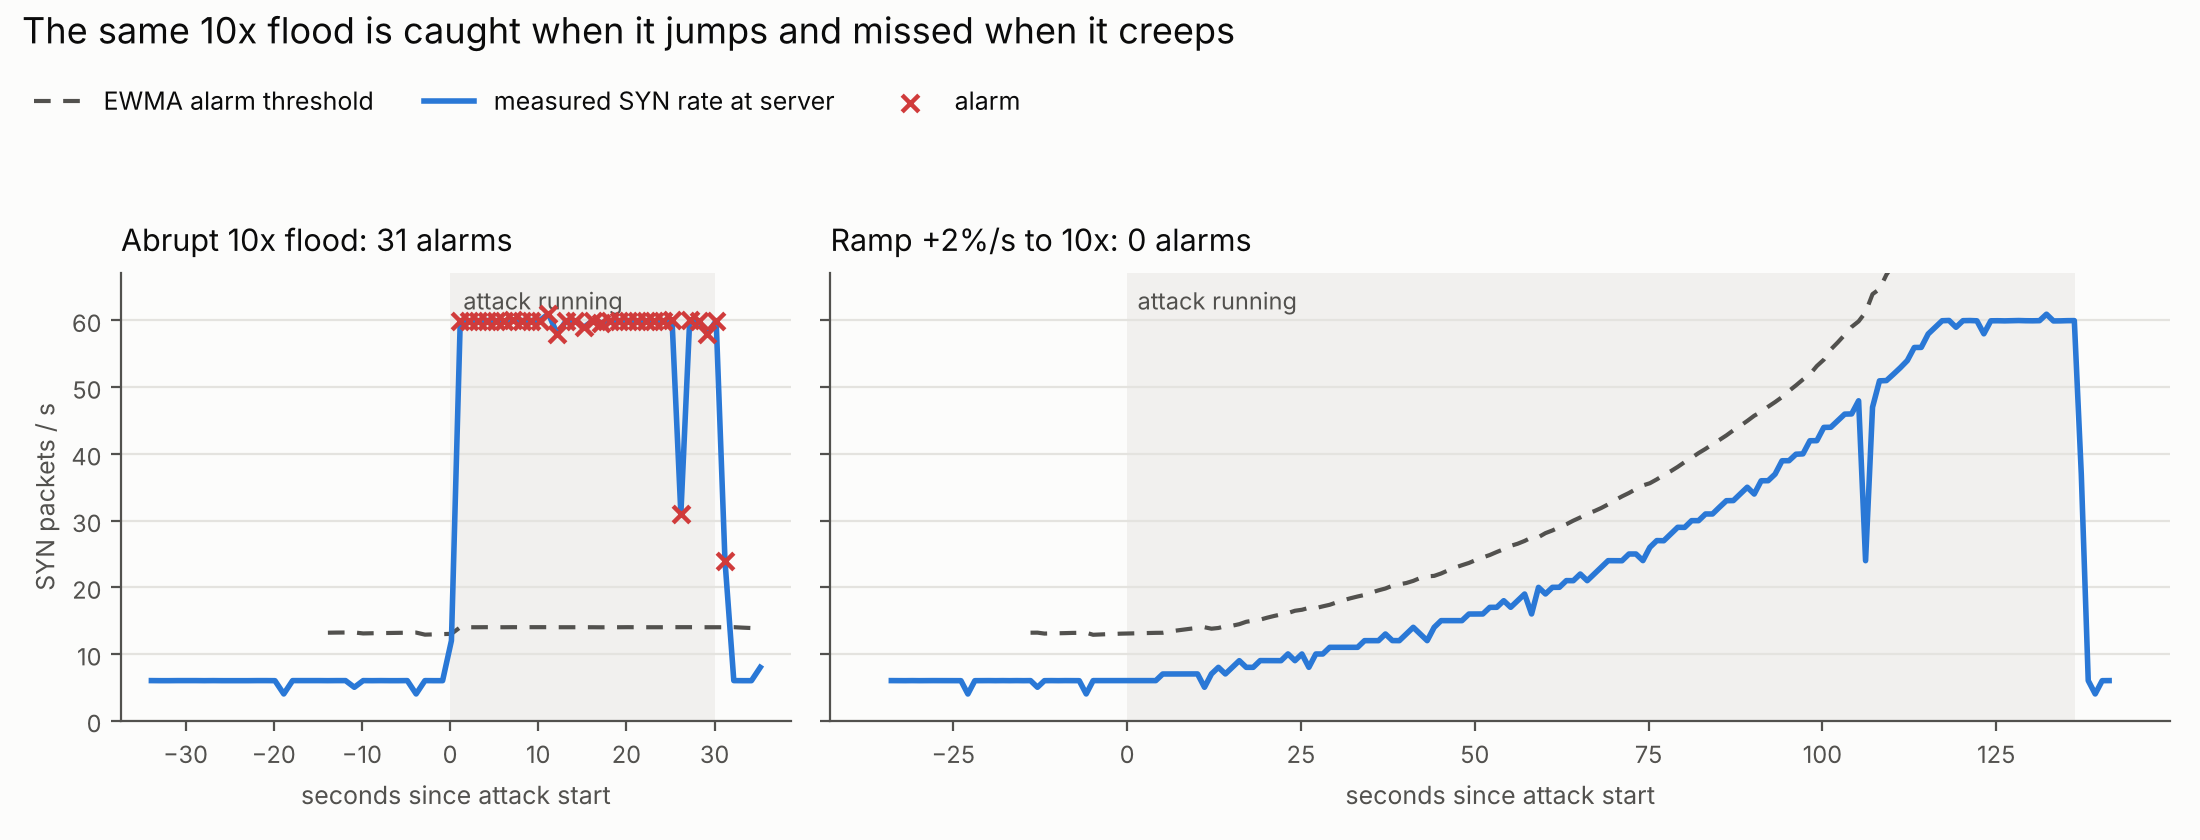
\includegraphics[width=0.95\linewidth]{step2_ramp_vs_abrupt.png}\\[1mm]
\begin{itemize}
\item The \textbf{same 10$\times$ SYN flood}: caught in about 1\,s when it jumps, \key{never caught} when it creeps up by 2\% per second.
\item Our attacker sends exactly what it plans: the switch counted 98--99\% of its packets.
\end{itemize}
\end{frame}

% ------------------------------------------------------------------ 4
\begin{frame}{Why this is hard: the detector's dilemma}
\begin{columns}[T]
\column{0.5\textwidth}
\textbf{Learn ``normal'' once, never again}\\[1mm]
{\small (Static: what our first version did)}
\begin{itemize}
\item[\textcolor{good}{\checkmark}] catches the slow attack
\item[\textcolor{bad}{$\times$}] \key{false alarm} whenever real users grow
\end{itemize}
\column{0.5\textwidth}
\textbf{Keep learning ``normal''}\\[1mm]
{\small (EWMA, Half-Space Trees = online machine learning)}
\begin{itemize}
\item[\textcolor{good}{\checkmark}] accepts real growth
\item[\textcolor{bad}{$\times$}] \key{learns the slow attack} as normal
\end{itemize}
\end{columns}
\vspace{6mm}
\begin{block}{The core observation}
Counting packets cannot tell a slow attack from a growing crowd of real users:
\textbf{in volume, they look the same}. We need a different kind of information.
\end{block}
\end{frame}

% ------------------------------------------------------------------ 5
\begin{frame}{Our idea: only learn from traffic the network can vouch for}
\begin{itemize}\setlength\itemsep{2.5mm}
\item Every visit to a website is a TCP connection: the client says \textbf{SYN} (``hello''),
      \dots, and at the end the server says \textbf{FIN} (``goodbye'').
\item \textbf{Real users finish their connections.} Fake (spoofed) SYNs never do.
\item So the switch counts two things and the controller divides:
\end{itemize}
\vspace{1mm}
\[
  \text{completion } e_n \;=\; \frac{\text{FINs sent by the server}}{\text{SYNs sent to the server}}
  \qquad\begin{cases} \approx 1 & \text{real users, even a sudden crowd}\\
                      \approx 1/m & \text{attack at } m\times \text{ the users' rate}\end{cases}
\]
\vspace{1mm}
\begin{itemize}
\item \key{Learning Gate:} the detector may update ``normal'' only while $e_n \ge \tau = 0.7$.
\item It never raises alarms itself. It only decides \emph{what the detector is allowed to learn}.
\end{itemize}
\end{frame}

% ------------------------------------------------------------------ 6
\begin{frame}{Why an attacker cannot fake the evidence}
\begin{itemize}\setlength\itemsep{3mm}
\item The FINs are counted \textbf{only on the switch port where the server's cable plugs in}.
      An attacker elsewhere cannot send packets that arrive on that cable.
\item Counting is done by \textbf{switch rules}, not by sending packets to the controller.
      The controller asks for the counters once a second, whatever the attack size.
      \aside{(Sending packets to the controller is itself a known weak spot of SDN.)}
\item Both counters use one switch feature: matching on \textbf{TCP flags}
      \aside{(an ONF extension to OpenFlow 1.3, standard in 1.5; Open vSwitch supports it)}
      (``SYN set, ACK clear'' $=$ a new connection; ``FIN set'' $=$ a finished one).
\end{itemize}
\end{frame}

% ------------------------------------------------------------------ 7
\begin{frame}{System architecture}
\vspace{-3mm}
\centering
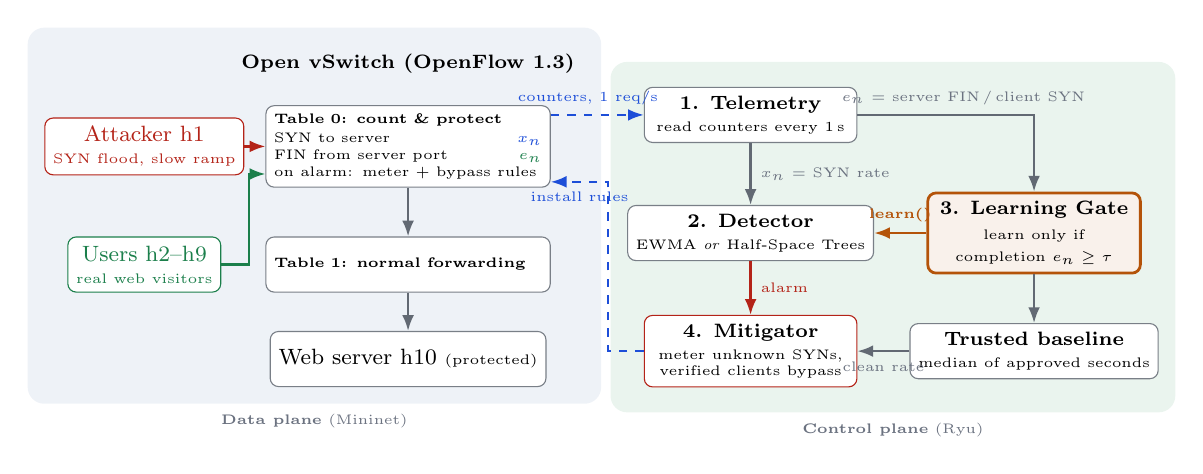
\begin{tikzpicture}[x=1cm,y=1cm]
\node[host, draw=bad, text=bad, minimum width=19mm] (bots) at (0.9,1.15) {\footnotesize Attacker h1\\\tiny SYN flood, slow ramp};
\node[host, draw=good, text=good, minimum width=19mm] (users) at (0.9,-0.35) {\footnotesize Users h2--h9\\\tiny real web visitors};
\node[tbl, text width=34mm] (t0) at (4.25,1.15) {%
  \textbf{Table 0: count \& protect}\\[1pt]
  SYN to server \hfill\textcolor{blue}{$x_n$}\\
  FIN from server port \hfill\textcolor{good}{$e_n$}\\
  on alarm: meter + bypass rules};
\node[tbl, text width=34mm] (t1) at (4.25,-0.35) {\textbf{Table 1: normal forwarding}};
\node[host, minimum width=34mm] (srv) at (4.25,-1.55) {\footnotesize Web server h10 \tiny(protected)};
\node[font=\scriptsize\bfseries] (ovs) at (4.25,2.2) {Open vSwitch (OpenFlow 1.3)};
\draw[arr, bad] (bots.east) -- (bots.east -| t0.west);
\draw[arr, good] (users.east) -- ++(0.35,0) |- ($(t0.west)+(0,-0.35)$);
\draw[arr] (t0.south) -- (t1.north);
\draw[arr] (t1.south) -- (srv.north);
\begin{scope}[on background layer]
  \node[zone, fill=plane, fit=(bots)(users)(ovs)(t0)(t1)(srv), inner ysep=6pt] (dp) {};
\end{scope}
\node[lbl, anchor=north] at (dp.south) {\textbf{Data plane} (Mininet)};
\node[stage] (poll) at (8.6,1.55) {\textbf{1. Telemetry}\\\tiny read counters every 1\,s};
\node[stage] (det)  at (8.6,0.05) {\textbf{2. Detector}\\\tiny EWMA \emph{or} Half-Space Trees};
\node[stage, draw=bad] (mit) at (8.6,-1.45) {\textbf{4. Mitigator}\\\tiny meter unknown SYNs,\\[-2pt]\tiny verified clients bypass};
\node[gatebox] (gate) at (12.2,0.05) {\textbf{3. Learning Gate}\\[1pt]
  \tiny learn only if\\ \tiny completion $e_n \ge \tau$};
\node[stage] (anchor) at (12.2,-1.45) {\textbf{Trusted baseline}\\\tiny median of approved seconds};
\draw[arr] (poll) -- node[lbl, right]{$x_n$ = SYN rate} (det);
\draw[arr, bad] (det) -- node[lbl, right, text=bad]{alarm} (mit);
\draw[arr] (poll.east) -| node[lbl, above, pos=0.3]{$e_n$ = server FIN\,/\,client SYN} (gate.north);
\draw[arr, gate, line width=1pt] (gate.west) -- node[lbl, above, text=gate]{\textbf{learn()}} (det.east);
\draw[arr] (gate) -- (anchor);
\draw[arr] (anchor.west) -- node[lbl, below]{clean rate} (mit.east);
\begin{scope}[on background layer]
  \node[zone, fill=ctrl, fit=(poll)(det)(mit)(gate)(anchor), inner ysep=9pt] (cp) {};
\end{scope}
\node[lbl, anchor=north] at (cp.south) {\textbf{Control plane} (Ryu)};
\draw[ctl] (t0.east |- poll.west) -- node[lbl, above, text=blue, pos=0.4]{counters, 1 req/s} (poll.west);
\draw[ctl] (mit.west) -- ++(-0.45,0) |- node[lbl, below, text=blue, pos=0.75]{install rules} ($(t0.east)+(0,-0.45)$);
\end{tikzpicture}
\end{frame}

% ------------------------------------------------------------------ 8
\begin{frame}{How we tested it}
\begin{columns}[T]
\column{0.5\textwidth}
\textbf{Network}
\begin{itemize}\small
\item 3 Open vSwitch switches, 12 hosts (Mininet)
\item Ryu controller, OpenFlow 1.3, two tables
\item Web server h10 with a realistic queue (511, the nginx default); every visitor treated as new
\end{itemize}
\textbf{Traffic}
\begin{itemize}\small
\item \textbf{Users}: \texttt{curl} every 0.5\,s from pools of 20 addresses per host
\item \textbf{Flash crowd}: users grow $5\times$ in 60\,s (no attack)
\item \textbf{Attackers}: h1, h11, h12 on three switches share spoofed SYNs, abrupt $10\times$ or a slow ramp
\end{itemize}
\column{0.5\textwidth}
\textbf{Detectors compared (all on the same numbers)}
\begin{itemize}\small
\item Static, EWMA, Half-Space Trees (online ML)
\item EWMA + gate, Half-Space Trees + gate
\end{itemize}
\textbf{Evaluation}
\begin{itemize}\small
\item 57 live runs (laptop, kernel datapath) + 12 runs after the fixes
\item 3--5 repeats per case, mean $\pm$ 95\% CI
\item $\tau$ and drift sweeps by replaying every recorded run offline
\end{itemize}
\end{columns}
\end{frame}

% ------------------------------------------------------------------ 9
\begin{frame}{Result 1: the gate catches the slow attack}
\centering
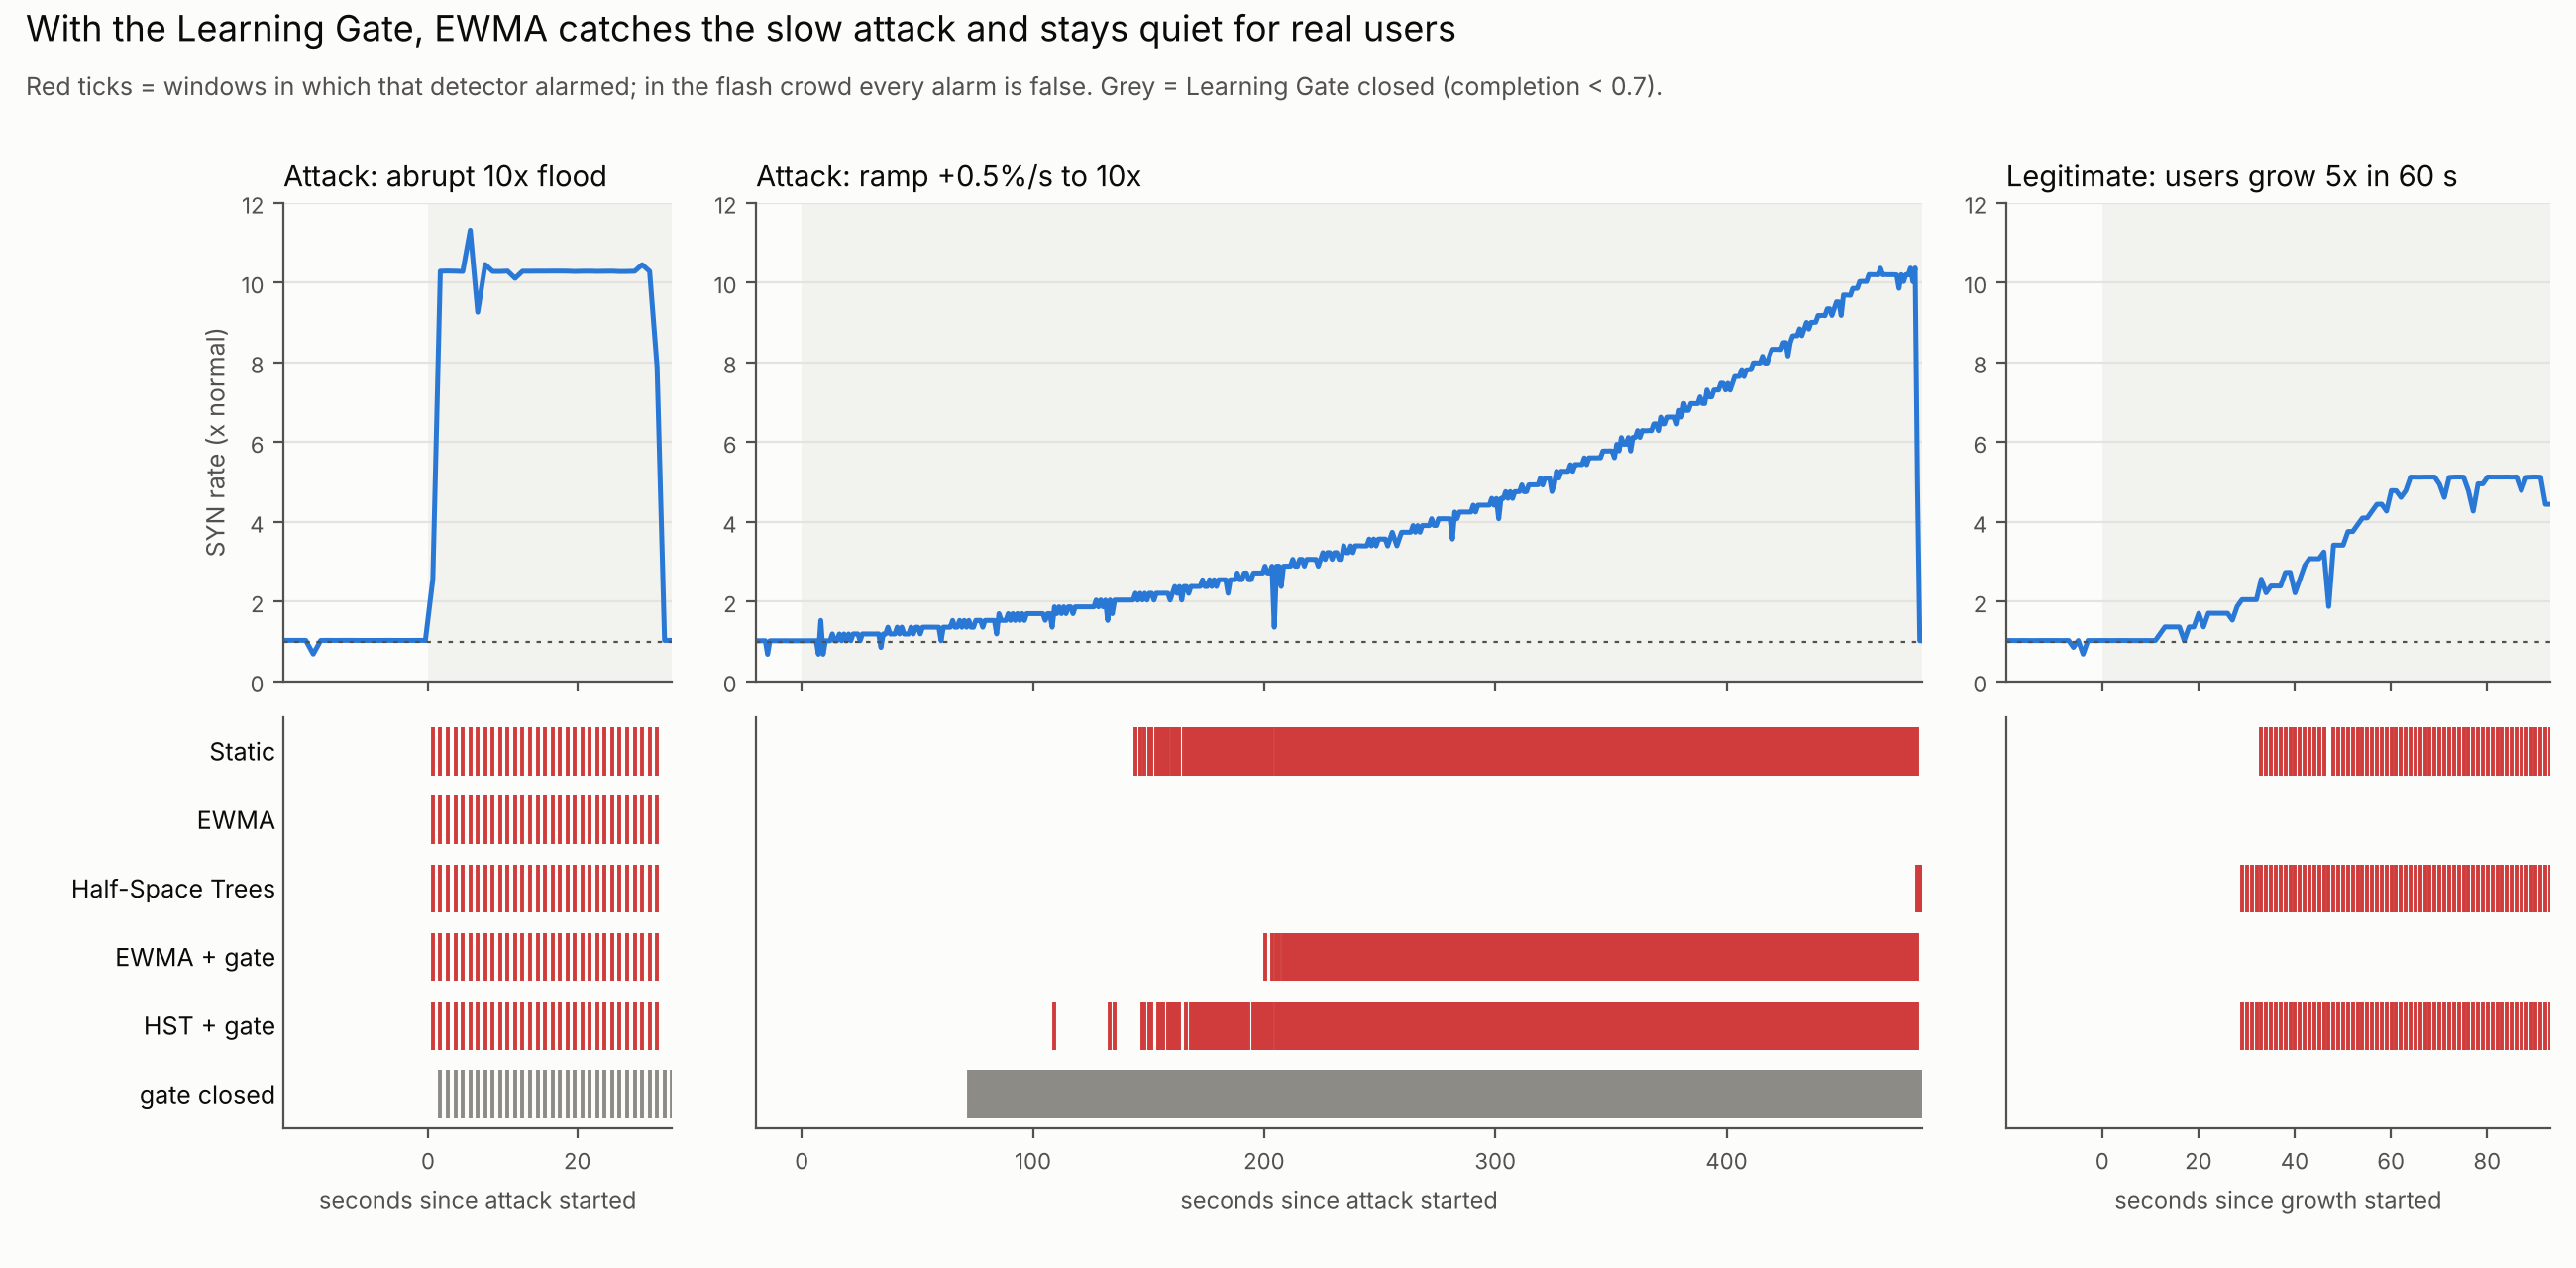
\includegraphics[height=0.74\textheight]{step4_detectors.png}\\
\aside{One live run of each scenario. Red = alarms; grey = gate closed. Repeated results on the next slide.}
\end{frame}

% ------------------------------------------------------------------ 10
\begin{frame}{Result 1 over repeated runs}
\centering\small
\begin{tabular}{lccc}
\toprule
 & \textbf{Abrupt 10$\times$ flood} & \textbf{Slow ramp (+0.5\%/s)} & \textbf{Real flash crowd} \\
 & caught & caught, at what size & false alarms \\
\midrule
Static           & 5/5 (1.1\,s) & 5/5 at 2.17$\times$ & \textcolor{bad}{5/5} \\
EWMA             & 5/5 (1.1\,s) & \textcolor{bad}{1/5} (at 10.2$\times$) & 1/5 \\
Half-Space Trees & 5/5 (1.1\,s) & \textcolor{bad}{1/5} & \textcolor{bad}{5/5} \\
\midrule
\textbf{EWMA + gate} & \textbf{5/5 (1.1\,s)} & \textbf{5/5 at 2.89$\times$ $\pm$ 0.11} & \textbf{1/5} \\
HST + gate       & 5/5 (1.1\,s) & 5/5 at 1.93$\times$ & \textcolor{bad}{5/5} \\
\bottomrule
\end{tabular}
\vspace{4mm}
\begin{itemize}\small
\item \key{EWMA + gate is the only detector that catches the slow attack without false alarms on real users.}
\item Same at +1\%/s (3/3 at 2.83$\times$) and +2\%/s (3/3 at 2.72$\times$); plain EWMA: 1/3 and 0/3.
\item The single crowd false alarm is EWMA's own (same run, with or without the gate).
\end{itemize}
\end{frame}

% ------------------------------------------------------------------ 11
\begin{frame}{Theory matches the network}
\begin{itemize}\setlength\itemsep{3mm}
\item With the attack at $m\times$ the users' rate, completion is about $1/m$.
      The gate closes when $1/m < 0.7$, i.e.\ at $m \approx \mathbf{1.43}$.
      \textbf{Measured: the gate closed at 1.43$\times$.}
\item After that, the detector's ``normal'' is frozen near 1.4$\times$, and its alarm line sits a
      few standard deviations above it.
      \textbf{Predicted alarm: about 2.9$\times$.\quad Measured: 2.89$\times$ $\pm$ 0.11 (5 runs).}
\item Without the gate: if the attacker keeps traffic a fraction $g$ above what an EWMA detector
      (learning weight $\beta$) has learned, ``normal'' grows by $(1+\beta g)$ every second, so
      reaching $F\times$ takes
      \[ n = \frac{\ln F}{\ln(1+\beta g)} \text{ seconds} \qquad
         (\beta = 0.1,\ g = 0.2:\ 10\times \text{ in } 116\,\text{s}),\]
      with \textbf{zero alarms}. Measured (ramp +2\%/s): 10.3$\times$, 0 alarms.
\end{itemize}
\end{frame}

% ------------------------------------------------------------------ 12
\begin{frame}{Step 2: stopping the attack without hurting users}
\begin{itemize}\setlength\itemsep{2.5mm}
\item The usual tool is a \textbf{SYN meter}: let at most $N$ new connections per second through.
      But during a $10\times$ flood about 9 in 10 SYNs are fake, so it \key{mostly blocks real users}.
\item Our evidence helps again: each FIN from the server \textbf{names a client that really
      finished a connection}. We call those clients \key{verified}.
\item On an alarm, the switch:
      \begin{itemize}
      \item gives each verified client a rule that \textbf{skips the meter};
      \item meters everything else to $1.5\times$ the trusted baseline.
      \end{itemize}
\item A spoofed address can never be verified: a spoofed SYN never completes.
\end{itemize}
\end{frame}

% ------------------------------------------------------------------ 13
\begin{frame}{Result 2: users are not slowed down, and the server's queue never fills}
\centering
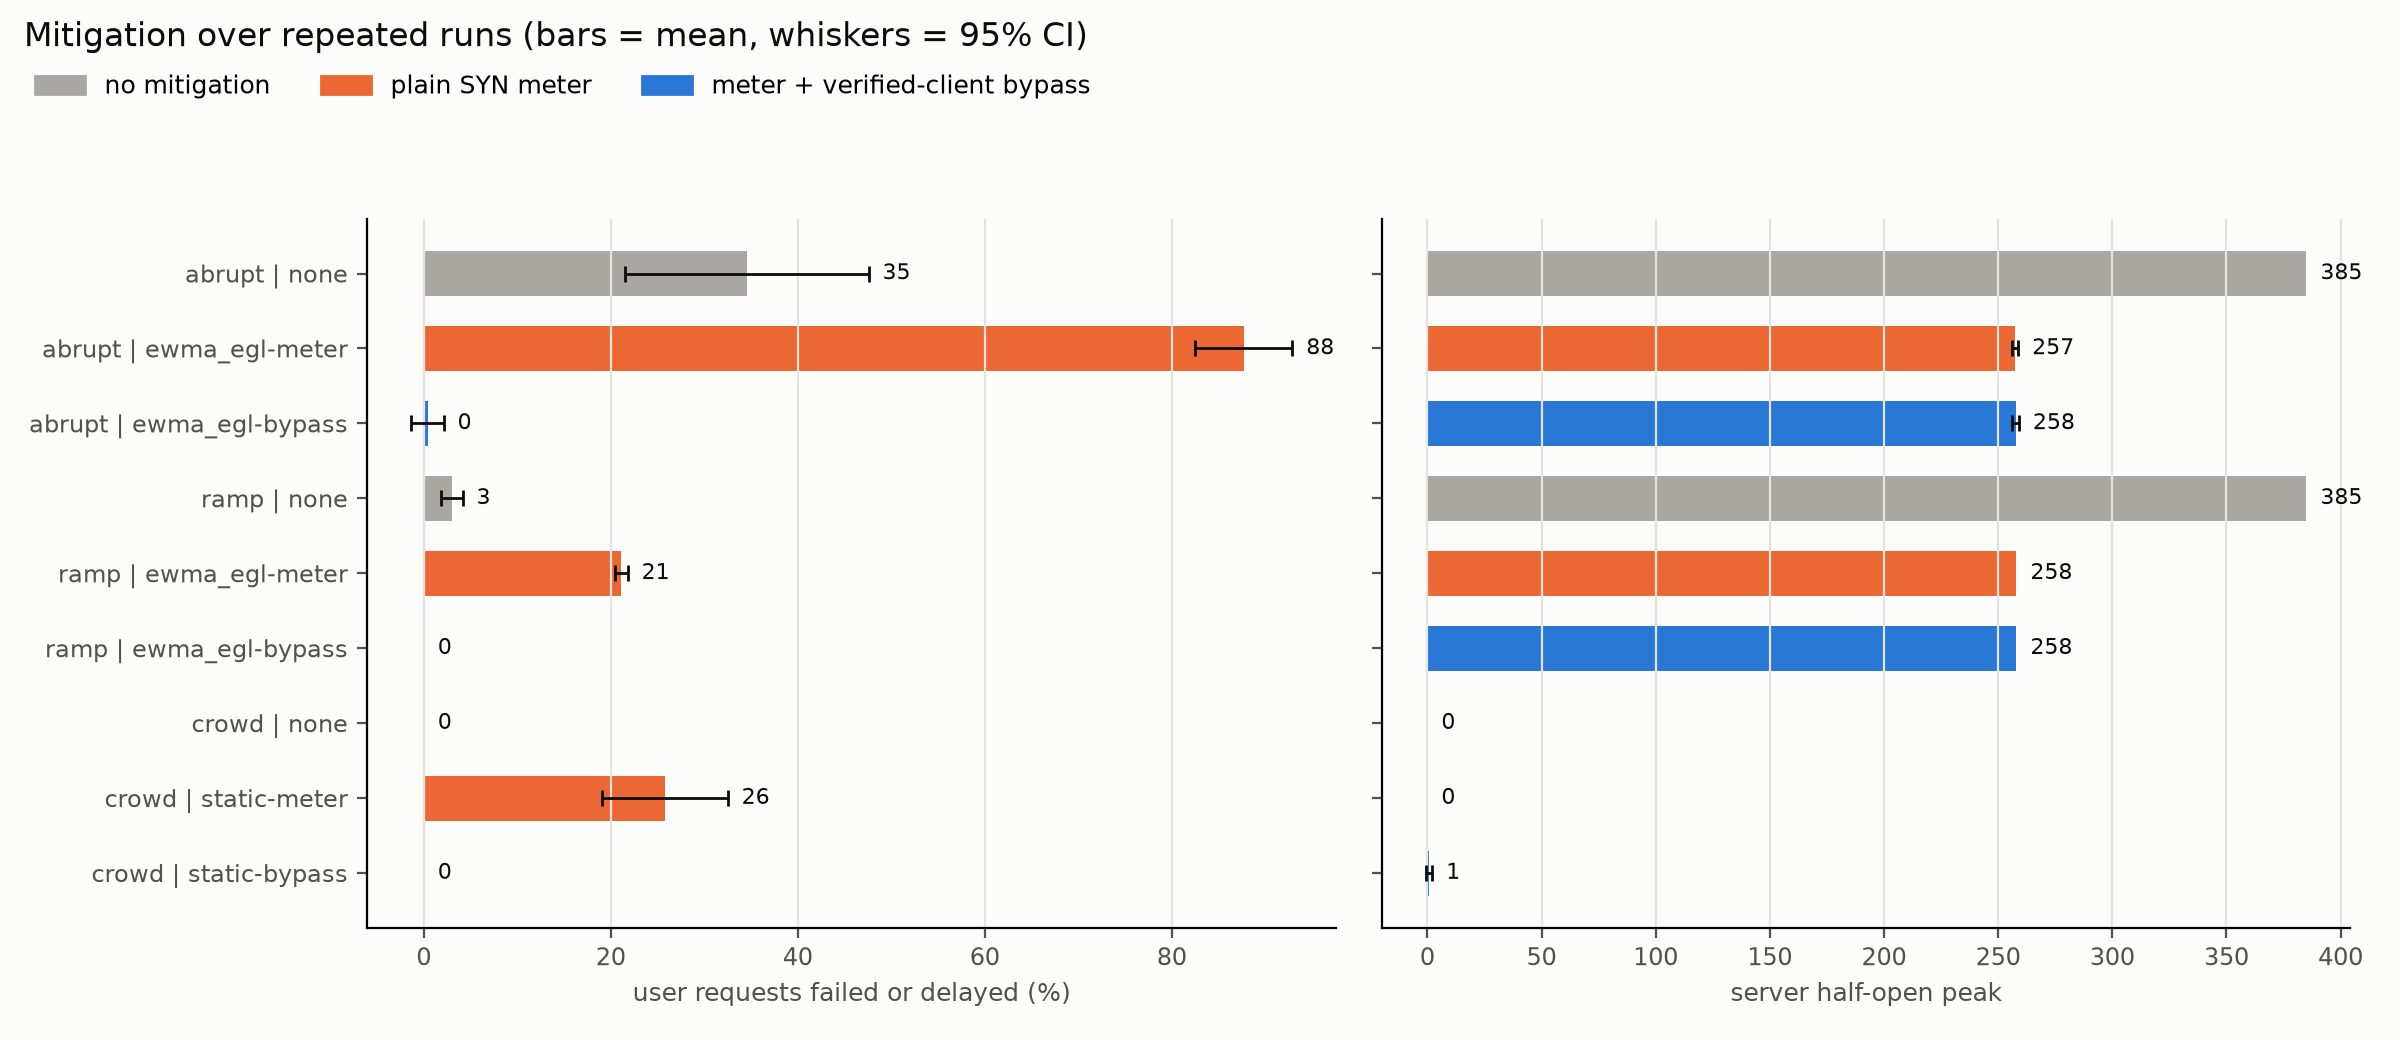
\includegraphics[width=0.86\linewidth]{fig_mitigation.png}\\
\small
Abrupt flood, 3 runs: requests failed or delayed --
\textcolor{muted}{none 34.5\%}, \textcolor{bad}{plain meter 87.7\%}, \textbf{bypass 0.4\%}.\\
Without mitigation the server's queue fills (385); with it, it stays at Linux's own limit ($\approx$258).
\end{frame}

\begin{frame}{Result 2, second by second}
\centering
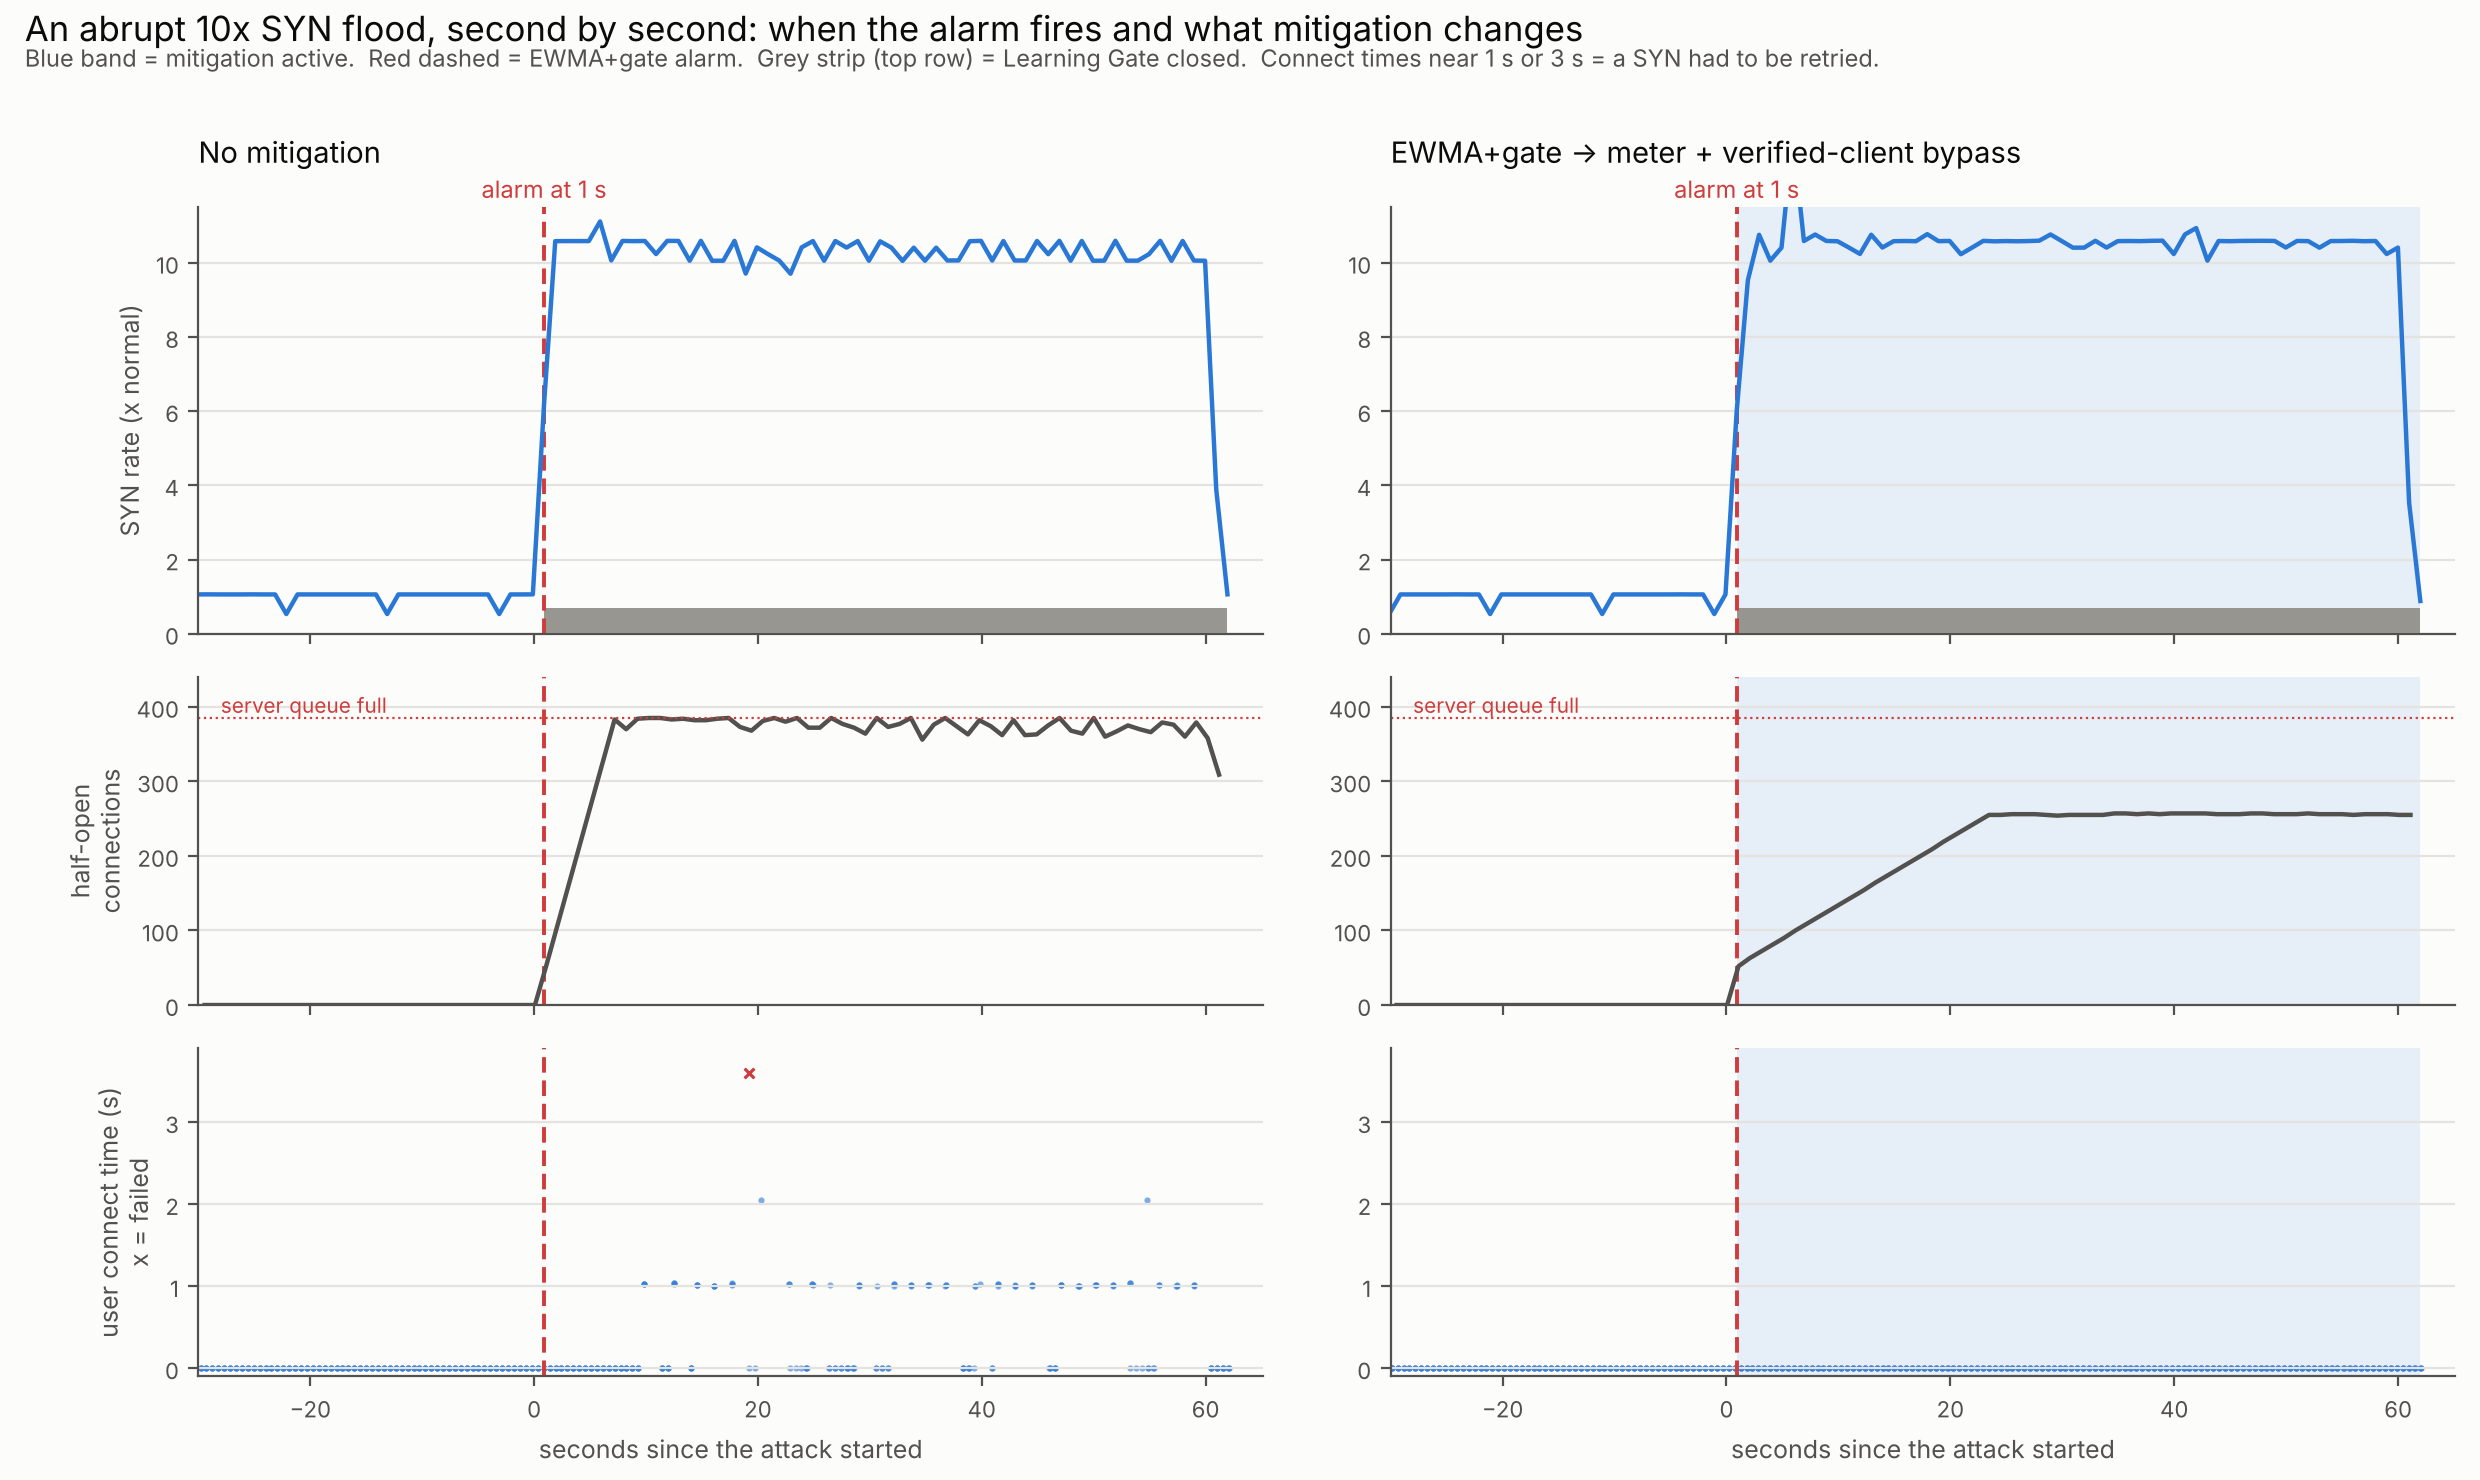
\includegraphics[height=0.64\textheight]{fig_timeline_abrupt.png}
\begin{itemize}\small
\item \textbf{Left, no mitigation:} the queue is full within 7\,s; about a third of users wait an extra 1--2\,s.
\item \textbf{Right, with bypass:} mitigation starts in the alarm's second (1\,s); the queue stays at
      Linux's own $\approx$258 level and every user connects instantly.
\end{itemize}
\end{frame}

% ------------------------------------------------------------------ 14
\begin{frame}{Fixed since the first version: attacks during warm-up}
\begin{itemize}\setlength\itemsep{2.5mm}
\item Every detector first watches for 60\,s to learn ``normal'' (\textbf{warm-up}). The network works
      normally meanwhile; only alarms are off.
\item \textbf{First version:} the gate guarded learning only \emph{after} warm-up. An attack that started
      during warm-up was learned as normal and never caught.
\item \textbf{Fix:} warm-up seconds count only when the gate accepts them. If the gate keeps rejecting,
      warm-up ends after 3$\times$ its length using the clean seconds it already has.
\end{itemize}
\vspace{2mm}
\centering\small
\begin{tabular}{lc}
\toprule
\textbf{10$\times$ flood starting 10\,s after the users} & \textbf{caught} \\
\midrule
Static, EWMA, Half-Space Trees & \textcolor{bad}{0/3} \\
EWMA + gate, \textbf{first version} & \textcolor{bad}{0/3} \\
\textbf{EWMA + gate, fixed} & \textbf{3/3} (49\,s after it starts) \\
HST + gate, fixed & 3/3 (49\,s) \\
\bottomrule
\end{tabular}\\[2mm]
\aside{Runs without an attack in warm-up are unchanged: replaying all 48 recorded results gives the same answers.}
\end{frame}

\begin{frame}{The attack is distributed: same results}
\centering\small
Validation runs with the attack split over three hosts (h1, h11, h12) on three switches:\\[3mm]
\begin{tabular}{lcc}
\toprule
 & \textbf{3 attacker hosts} & \textbf{1 attacker host (main runs)} \\
\midrule
Abrupt 10$\times$: caught by every detector & 2/2, $\approx$1\,s & 5/5, 1.1\,s \\
Ramp +1\%/s: EWMA + gate & \textbf{2/2 at 3.09$\times$} & 3/3 at 2.83$\times$ \\
Ramp +1\%/s: plain EWMA & 0/2 & 1/3 \\
Completing bots: EWMA + gate & 0/1 & 0/3 \\
Bypass: users failed or delayed & 0.7\% (none: 20.6\%) & 0.4\% (none: 34.5\%) \\
\bottomrule
\end{tabular}\\[3mm]
\aside{The detector watches total traffic reaching the server, so how many machines send it does not matter.}
\end{frame}

\begin{frame}{Choosing the threshold $\tau$}
\centering
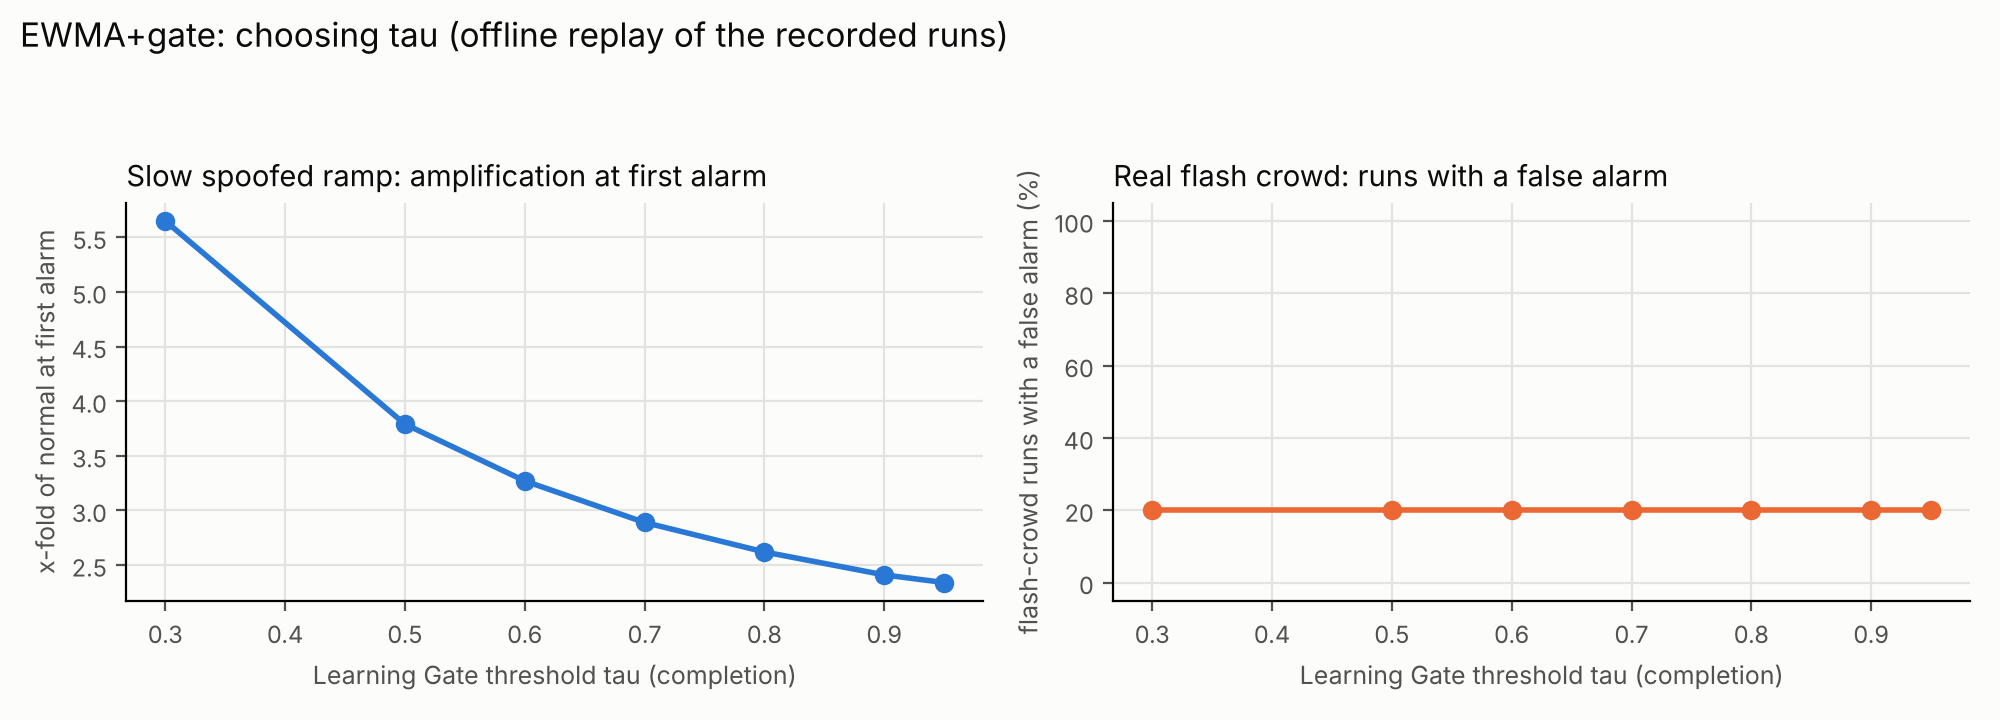
\includegraphics[width=0.95\linewidth]{fig_tau.png}
\begin{itemize}\small
\item A higher $\tau$ freezes learning earlier, so the attack is caught smaller (5.7$\times$ at 0.3 down to 2.3$\times$ at 0.95).
\item Real crowds keep completion near 1, so the false-alarm rate does not change with $\tau$. We use $\tau = 0.7$.
\end{itemize}
\end{frame}

% ------------------------------------------------------------------ 15
\begin{frame}{What it does not solve (honest limits)}
\begin{itemize}\setlength\itemsep{2.5mm}
\item \textbf{Bots that complete real connections} (an application-layer flood) look like real users.
      EWMA + gate missed them in 3 of 3 runs. That needs application-level defences.
\item A \textbf{drift budget} (``never learn faster than $\delta$ per second'') catches those bots
      (3/3 for $\delta \le 2\%$/s), but then \key{false-alarms on every real flash crowd} (5/5). A trade-off, not a fix.
\item The gate fixes \textbf{what a detector learns}, not \textbf{how it alarms}: Half-Space Trees still
      false-alarms on crowds with the gate.
\item \textbf{Brand-new visitors} arriving mid-attack must pass the meter before they are verified.
\item Small testbed: at this scale Linux itself survives a 10$\times$ flood (users are delayed, not refused).
\end{itemize}
\end{frame}

% ------------------------------------------------------------------ 16
\begin{frame}{Summary}
\begin{enumerate}\setlength\itemsep{3mm}
\item \textbf{The attack:} adaptive SDN DDoS detectors can be slowly ``boiled'': a 10$\times$ flood
      went unnoticed. First study of this for SDN, with a formula for how fast it works.
\item \textbf{The fix:} \key{Evidence-Gated Learning}: a detector may learn only from traffic the
      server actually completes. Works with any learning detector, uses only switch counters,
      and cannot be faked from outside.
\item \textbf{The result:} slow attack caught at 2.89$\times$ in 5/5 runs, real crowds accepted;
      with verified-client bypass the server is protected and real users see no delay.
\end{enumerate}
\vspace{5mm}
\aside{Code, data and every figure: \texttt{github.com/Anirudh-N-15/mininet}, branch \texttt{egl}.}
\end{frame}

\end{document}
